%%%%%%%%%%%%%%%%%%%%%%%%%%%%%%%%%%%%%%%%%%%%%%%%%%%%%%%%%%%%%%%%%%%%%%%%%%%%%%%%
\chapter{Анализ систем мониторинга и постановка задачи}
%%%%%%%%%%%%%%%%%%%%%%%%%%%%%%%%%%%%%%%%%%%%%%%%%%%%%%%%%%%%%%%%%%%%%%%%%%%%%%%%
В настоящее время существует большое количество программных комплексов
мониторинга систем в различных областях. В рамках данной работы интерес представляют системы, использование которых было бы целесообразно для проведения мониторинга СХД.
Средства, с помощью которых можно осуществлять мониторинг параметров систем хранения данных можно разделить на две группы:
\begin{itemize*}
	\item{Специальные системы}
	\item{Системы мониторинга общего назначения}
\end{itemize*}
Рассмотрим подробнее каждую группу.
 
%%%%%%%%%%%%%%%%%%%%%%%%%%%%%%%%%%%%%%%%%%%%%%%%%%%%%%%%%%%%%%%%%%%%%%%
\section{Специальные системы мониторинга}
Представителями первой группы являются продукты фирм IBM, EMC и FUJITSU. Данные системы разработаны самими  производителями систем хранения данных и чаще всего поставляются в комплекте с СХД.

\subsection{IBM Spectrum}
Система мониторинга параметров СХД поставляемая с оборудованием IBM. Позволяет нотифицировать об изменении состояния компонента и отслеживать состояние компонентов визуально. Пользовательский интерфейс системы представлен на рисунке~\ref{fig:Spectrum}.
\begin{figure}[!h]
	\centering
	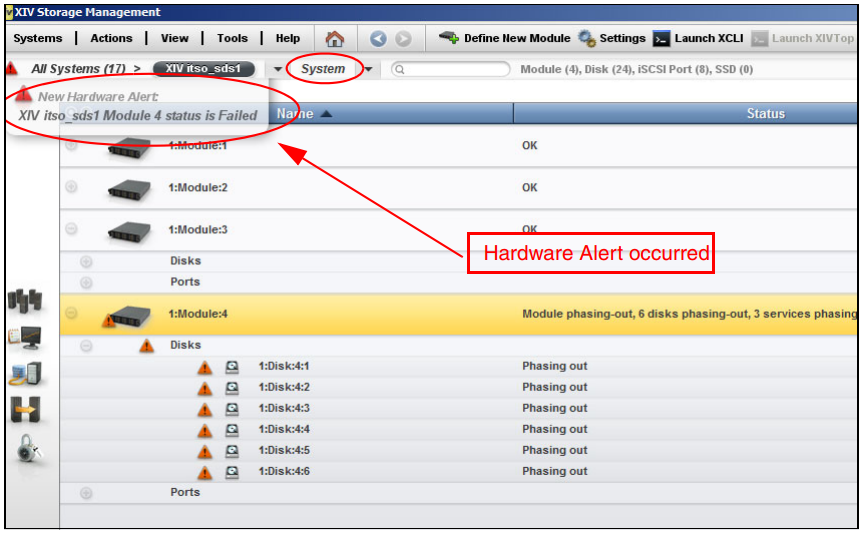
\includegraphics[width=\textwidth]{Spectrum}
	\caption{Пользовательский интрефейс IBM Spectrum}
	\label{fig:Spectrum}
\end{figure}

В системе предполагается градация по пяти уровням критичности произошедшего события~\cite{Spectrum}. Уровни градации представлены на рисунке~\ref{fig:Spectrum2}.
\begin{figure}[!h]
	\centering
	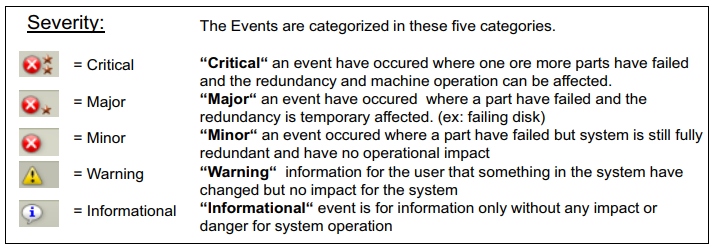
\includegraphics[width=\textwidth]{Spectrum2}
	\caption{Градация сообщений системы Spectrum}
	\label{fig:Spectrum2}
\end{figure}
Среди достоинств системы можно отметить широкую классификацию событий и понятный пользователю интерфейс. Однако, система не обладает возможностью присылать уведомления  админимтратору на почту/смс, а значит требует постоянного присутствия человека. Вторым недостатком системы является большая ориентированность на скоростные, стоимостные и нагрузочные показатели, нежели на характеристику компонентов и системы в целом. 
\subsection{EMC VNX Monitoring and Reporting}
Система мониторинга и информирования от EMC~\cite{EMC}, предоставляемая совместно с оборудованием. Позволяет в графическом виде наблюдать структуру системы, нагрузку на компоненты, активность сервисов системы. 
\begin{figure}[!h]
	\centering
	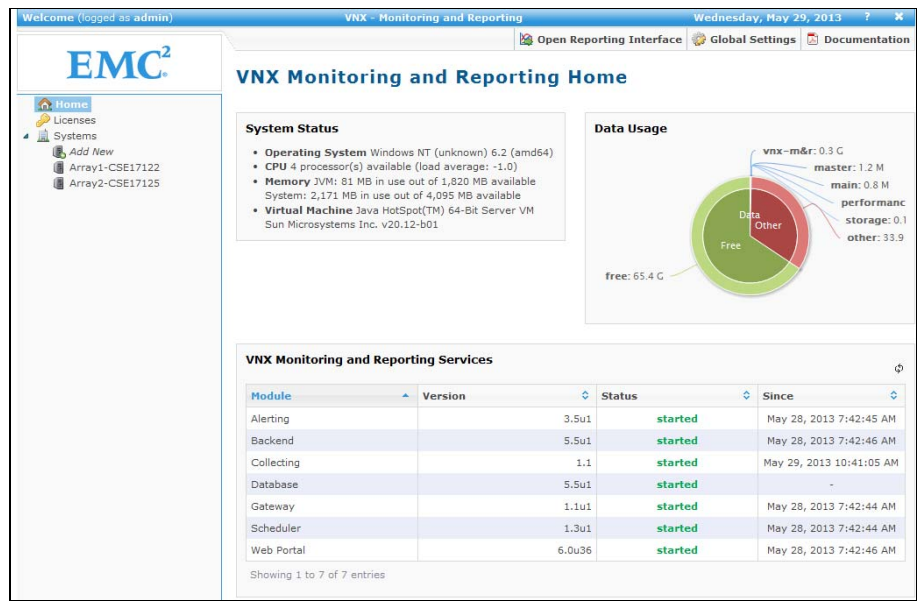
\includegraphics[width=\textwidth]{EMC}
	\caption{Пользовательский интрефейс EMC VNX}
	\label{fig:EMC}
\end{figure}
Аналогично системе Spectrum, используются информирующие сообщения пяти уровней критичности, но имеется возможность уведомления о событиях на электронную почту. Кроме того, в системе присутствует большое количество сетевых и системных настроек, позволяющих создавать кластеры, размечать диски, настраивать доступы и сети. Таким образом, система является в большей степени комплексной,а задача мониторинга состояния компонентов не является основопологающей. 

\subsection{FUJITSU ServerView System Monitor}
Еще одна специальная система мониторинга разработана компанией FUJITSU~\cite{Fujitsu}. Является визуализатором дерева подкомпонентов системы с состоянием каждого. Пользовательский интерфейс представлен на рисунке~\ref{fig:Fujitsu}.  
\begin{figure}[!h]
	\centering
	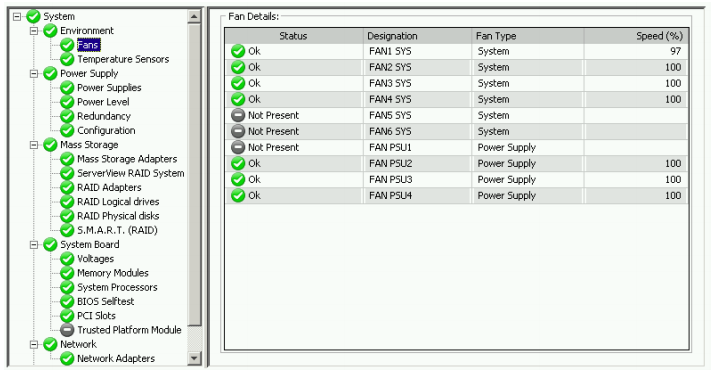
\includegraphics[width=\textwidth]{Fujitsu}
	\caption{Пользовательский интрефейс FUJITSU Server View}
	\label{fig:Fujitsu}
\end{figure}
Кроме десктопного исполнения FUJITSU разработала мобильное приложение, с аналогичной функциональностью (см. рисунок ~\ref{fig:Fujitsu2}).
\begin{figure}[!h]
	\centering
	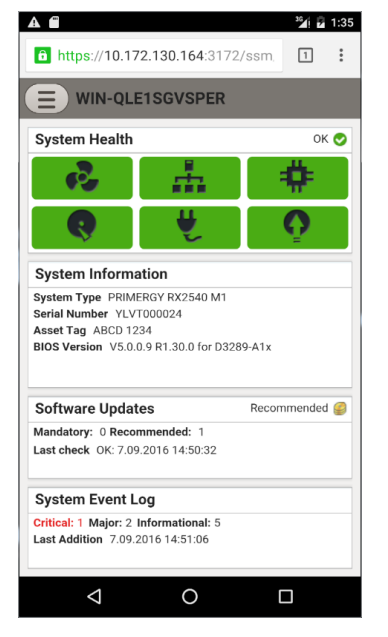
\includegraphics[width=2.0in]{Fujitsu2}
	\caption{Мобильное приложение от Fujitsu}
	\label{fig:Fujitsu2}
\end{figure}

Преимуществом данной системы по сравнению с ранее рассмотренными является большее уделение внимания состоянию системы в целом и компонентов в частности. Дерево компонентов системы позволяет быстро оценить состояние каждого,а при необходимости раскрыть и узнать большее количество информации, вплоть до причины возникновения ошибки. Кроме того, разработанное мобильное приложение позволяет администратору быть в курсе событий даже если он не находится непосредственно на рабочем месте. 
%%%%%%%%%%%%%%%%%%%%%%%%%%%%%%%%%%%%%%%%%%%%%%%%%%%%%%%%%%%%%%%%%%%%%%%
\section{Системы мониторинга общего назначения}
Представителями второй группы являются Elastic, Zabbix, Anomaly и др. Данные системы разрабатываются отдельно от систем хранения данных и предназначены для решения более общих задач, таких как сбор данных с большого количества источников, обработка данных, визуализация и поиск аномалий. 

\subsection{Elastic}

Система Elastic представляет из себя свободно распространяемый стек программ, предназначенный для сбора, хранения, обработки и отображения данных из разных источников. 
Состав программных продуктов Elastic представлен ниже: 
\begin{itemize*}
	\item{Elasticsearch – поисковая система с открытым исходным кодом, использует REST интерфейс и оперирует данными в формате JSON}
	\item{Kibana – инструмент позволяющий визуализировать данные в виде графиков, статистики и пр.}
	\item{Logstash - конвейер обработки данных на стороне сервера, который получает данные из нескольких источников одновременно, преобразует их, а затем отправляет в хранилище, например Elasticsearch}
	\item{Beats - платформа для легковесной отправки данных. Существует возможность отправлять данные с тысяч машин и систем в Logstash, используется для сбора данных}
	\item{ECE - Elastic Cloud Enterprise – предоставляет доступ для управления и контроля Elasticsearch и Kibana в любой инфраструктуре, управляя всем с одной консоли}
	\item{Machine learning – часть программного пакета X-Pack. Основной возможностью продукта является обнаружение аномалий временных рядов с использованием машинного обучения.}
\end{itemize*}

Наиболее интересным с точки зрения мониторинга параметров является последний пакет. Наилучшим применением данной технологии является обнаружение отклонений в значениях некоторых величин от нормального поведения. Чаще всего для этих целей используют правила, пороговые значения и различные простые статические методы. Однако такие способы зачастую неэффективны, так как они основываются на неверных статистических допущениях (Гауссово распределение и др.), а также не учитывают тренды (долгосрочное или периодическое изменение сигнала). Еще одним преимуществом пакета является возможность совместного анализа большого количества метрик, выявляя неявные зависимости. Предоставляется возможность вывода информации о всех аномалиях на один общий график. Анализ данных производится в реальном времени, возможно оповещение об обнаруженных аномалиях. Пакет полностью бесплатен начиная с 7 сентября 2018 года. 


\begin{figure}[htbp]
	\centering
	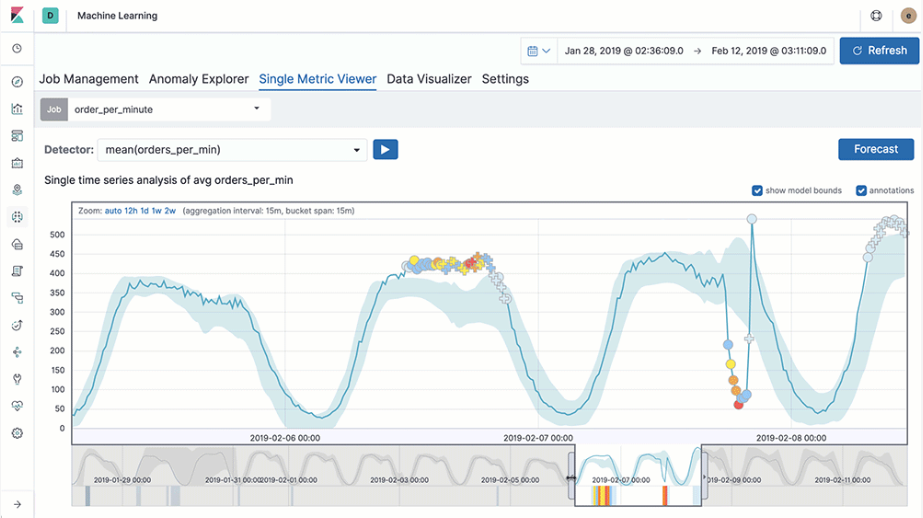
\includegraphics[width=\textwidth]{Elastic}
	\caption{Обнаружение аномалий в Elastic}
	\label{fig:Elastic}
\end{figure}

\subsection{Zabbix}

Zabbix - это программное обеспечение для мониторинга параметров сети, жизнеспособности и целостности серверов. Zabbix состоит из нескольких компонентов:
\begin{itemize*}
	\item{сервер мониторинга, который выполняет периодическое получение данных, обработку, анализ и запуск скриптов оповещения}
	\item{агенты - демоны, которые запускаются на отслеживаемых объектах и предоставляет данные серверу}
	\item{база данных (MySQL, PostgreSQL, SQLite или Oracle) для хранения накопленной информации}
	\item{веб-интерфейс на PHP, предоставляющий информацию о производительности и состоянии системы}
\end{itemize*}

\begin{figure}[!htbp]
	\centering
	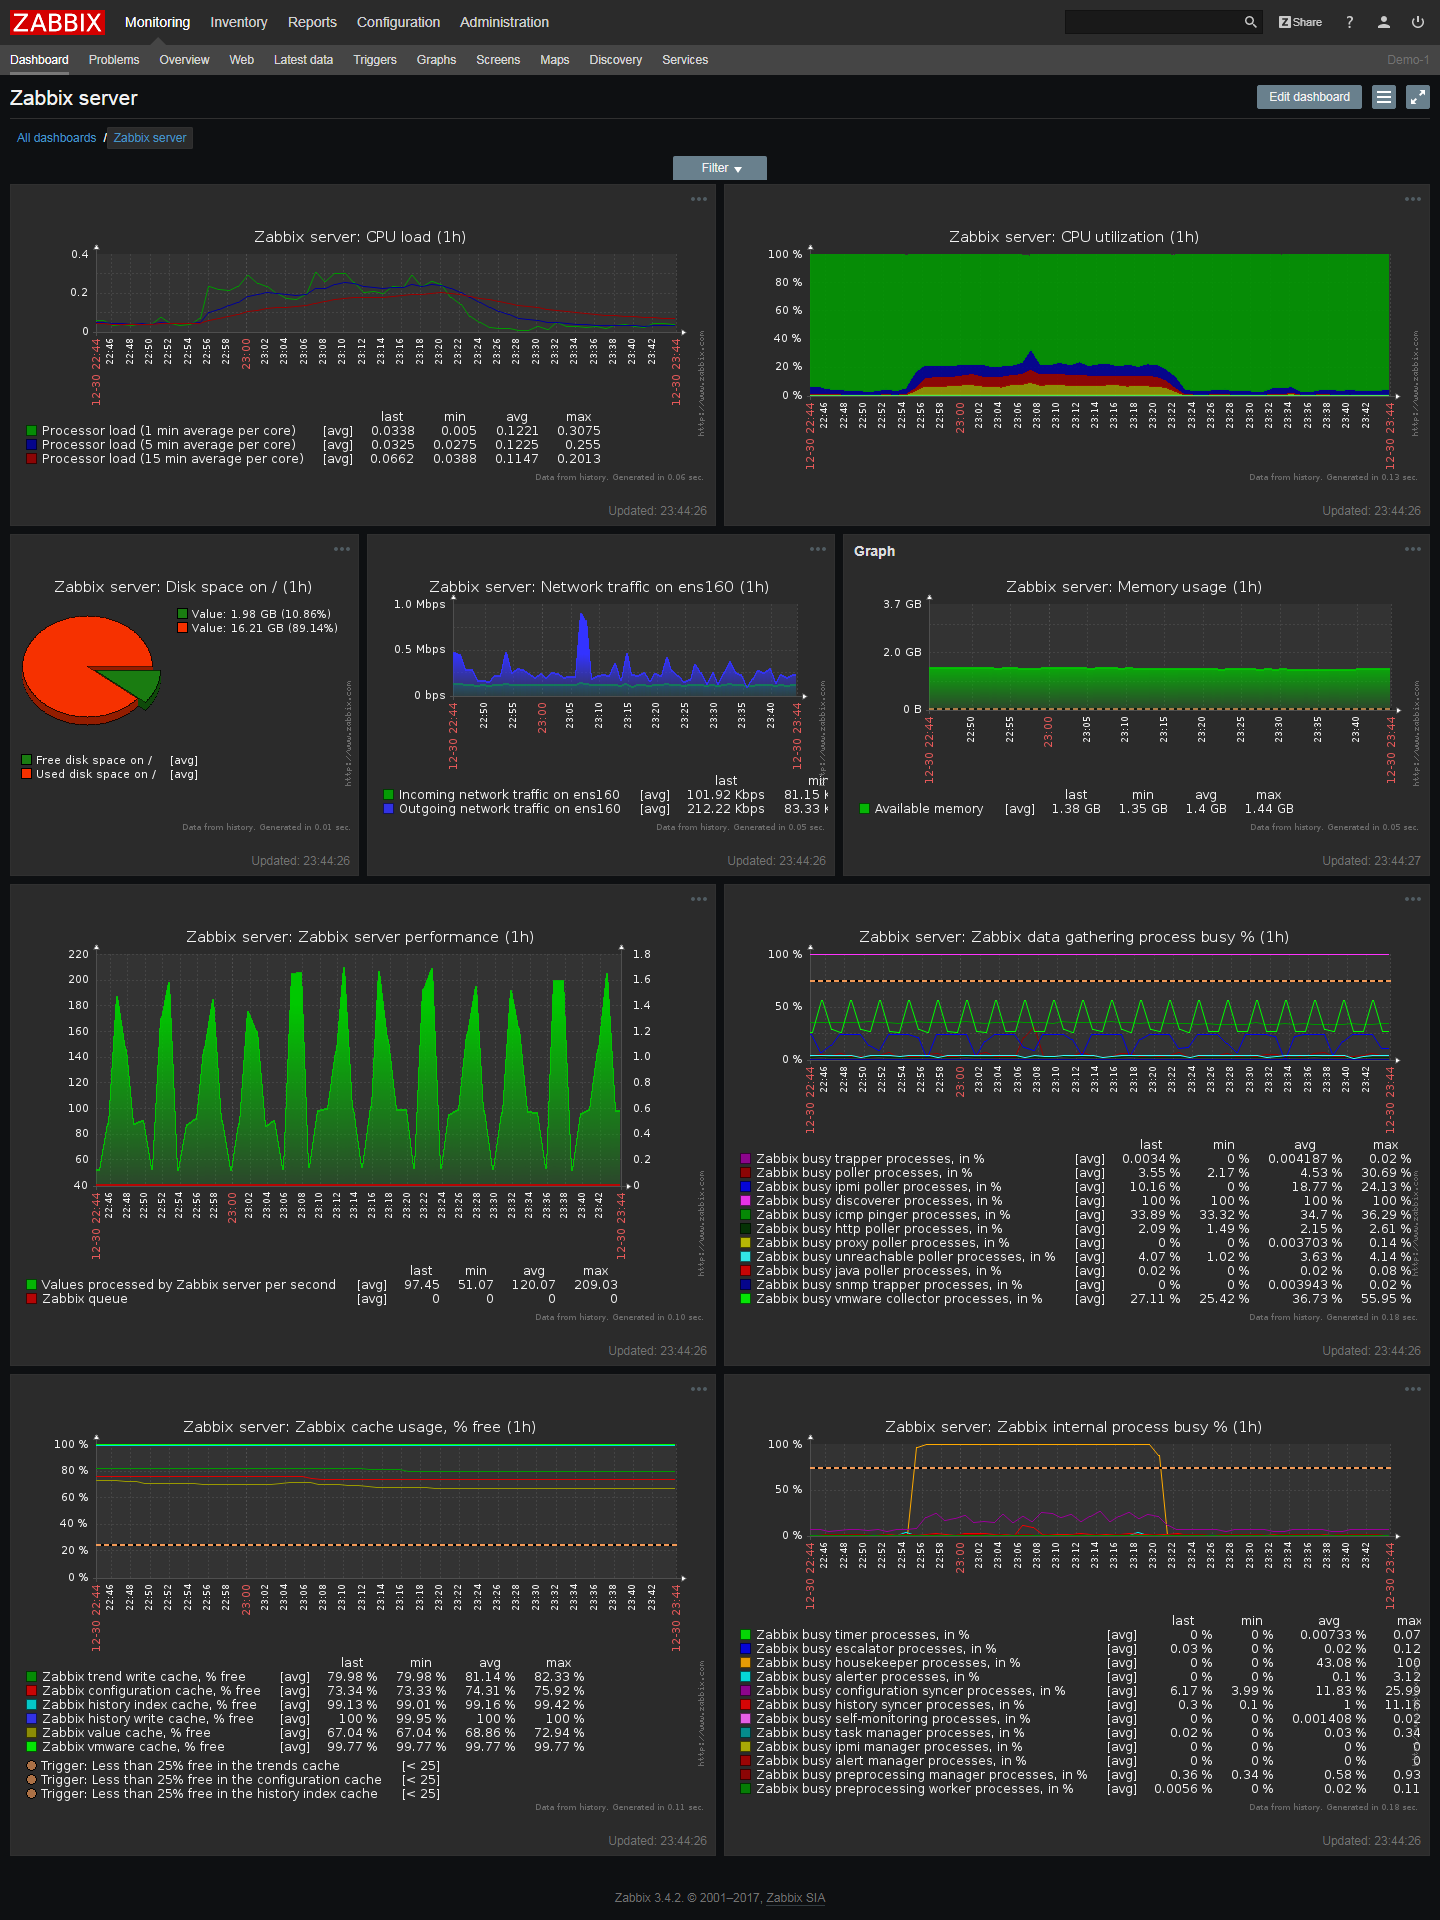
\includegraphics[width=\textwidth]{Zabbix}
	\caption{Отображение парметров в графическом виде в системе Zabbix}
	\label{fig:Zabbix}
\end{figure}

Преимуществом системы является возможность работаты без агента. Для этого используются общие протоколы мониторинга, такие как протокол управления сетью.  Кроме того, мониторинг можно производить с помощью запуска внешних скриптов, встроенных проверок (http запрос, ping и др). Недостатком системы явялется то, что продукт является коммерческим, а значит нет возможности собственной доработки и его продажи совместно с другими собственными продуктами.  

\subsection{Anomaly} 
Anomaly представляет из себя сервис по диагностированию аномалий в реальном времени~\cite{Anomaly}. Данные для мониторинга загружаются в облако, где после обработки и процесса обучения становится доступным детектирование отклонений в поведении (см. рисунок ~\ref{fig:Anomaly}). При этом процесс обучения не останавливается и длится постоянно. После первичного обучения алгоритмы формируют простые паттерны определения ошибок, такие как максимумы и минимумы. Со временем происходит детализирование и выявление корреляций, трендов и др. Для обучения используется машинное обучение, нейронные сети, собственные математические модели. 
\begin{figure}[!h]
	\centering
	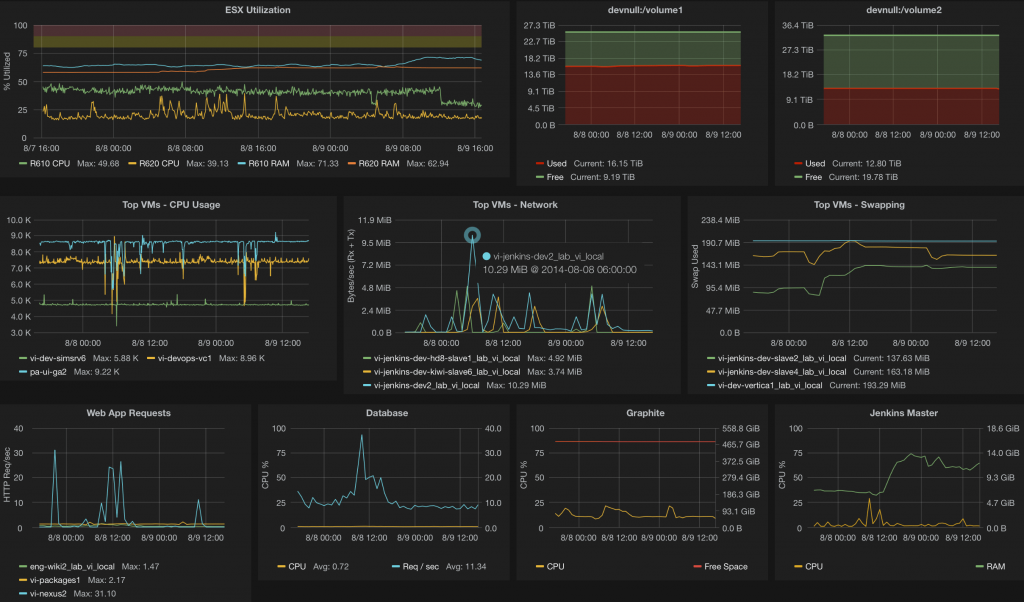
\includegraphics[width=\textwidth]{Anomaly}
	\caption{Пользовательский интерфейс Anomaly}
	\label{fig:Anomaly}
\end{figure}

При обнаружении аномалии пользователю отправляется сообщение (смс, почта) или выполняется собственно-назначенное действие. Система является коммерческим продуктом. Недостатком системы является удаленное расположение сервера обработки данных. В случае закрытых ЦОД или иных ограниченных доступом систем данное решение не применимо. Кроме того, в случае использования такой системы появляется необходимость транзита большого количества данных по сети, что увеличивает загрузку на сеть. Однако, использование сторонних серверов для обработки данных позволеяет экономить собсвтенные вычислительные ресурсы. 

\section{Постановка задачи}

Резюмируя вышесказанное можно заключить, что существует большое количество различных систем мониторинга параметров, однако они обладают рядом недостатков:
\begin{itemize*}
	\item{Системы, поставляющиеся с оборудованием от производителя, работают только с их оборудованием, и, зачастую, не отображают данные в удобном виде}
	\item{Системы общего назначения максимально унифицированы под сбор и визуализацию всевозможных данных, поэтому такие системы не отображают иерархически компоненты системы, что усложняет определение последствий возникновения аномалий.  Кроме того, зачастую такие системы расположены на удаленных серверах, что делает невозможным их применение в закрытых(изолированных) решениях.}
\end{itemize*}

Таким образом, актуальной является задача разработки собственной системы мониторинга и диагностики СХД. В рамках одного из проектов научной лаборатории НИЛ АСПОД в СПбПУ разрабатывается такая система. Структура разрабатываемой системы приведена на рисунке ~\ref{fig:diagSystem}.
\begin{figure}[!h]
	\centering
	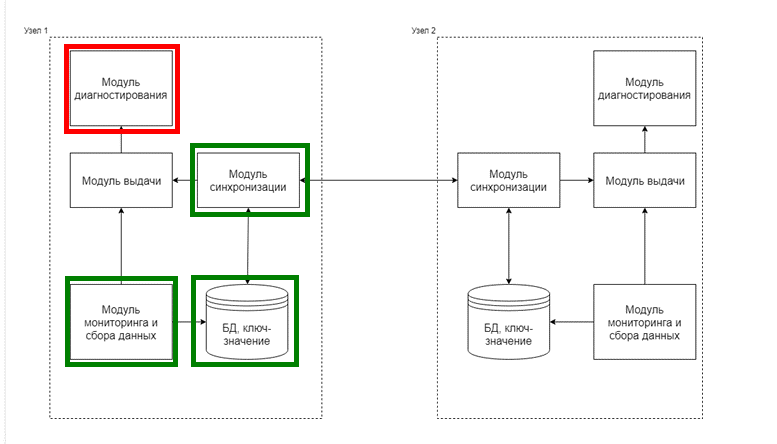
\includegraphics[width=\textwidth]{diagSystem}
	\caption{Структура разрабатываемой в лаборатории системы мониторинга и диагностики}
	\label{fig:diagSystem}
\end{figure}

Зеленым цветом выделены ранее реализованные модули, в данной работе рассматривается ряд прикладных задач в рамках работы над модуелем диагностирования. В частности, формулируется задача описания методики диагностики состояний системы хранения данных, что предполагает решенеие ряда задач:
\begin{itemize*}
	\item{Анализ параметров для диагностики дисков}
	\item{Описание методологии ????}
\end{itemize*}
Кроме того, с целью обеспечения полноты собираемых параметров, формулируется задача разработки и изготовления аппаратно-программного комлекса сбора и отображения климатических параметров СХД. Для достижения поставленной цели необходимо решить ряд задач: 
\begin{itemize*}
	\item{Разработка структуры комплекса}
	\item{Разработка и реализация аппаратной части}
	\item{Разработка и реализация программной части}
\end{itemize*}	 

%%\begin{table}
% Для таблиц с multirow и multicol необходимо вручную указать сдвиг для caption
%%\captionsetup{skip=5pt}
%%\caption{Example}
%%\centering
%%\begin{tabular}{|r|c|c|c|c|c|c|}
%%\hline
%%            \multirow{2}{*}{}
%%           & \multicolumn{2}{c|}{LLVM IR} 
%%           & \multicolumn{2}{c|}{PS} 
%%           & \multicolumn{2}{c|}{AI} \\ \cline{2-7}
%%           & SAT    & UNSAT   & SAT    & UNSAT   & SAT    & UNSAT   \\ \hline
%%beanstalkd & 356    & 252     & 360    & 161     & 360    & 247     \\ \hline
%%clib       & 599    & 258     & 960    & 234     & 960    & 449     \\ \hline
%%\end{tabular}
%%\label{table:checkResults}
%%\end{table}

%%%%%%%%%%%%%%%%%%%%%%%%%%%%%%%%%%%%%%%%%%%%%%%%%%%%%%%%%%%%%%%%%%%%%%%%%%%%%%%%
%%\section{bar}
%%%%%%%%%%%%%%%%%%%%%%%%%%%%%%%%%%%%%%%%%%%%%%%%%%%%%%%%%%%%%%%%%%%%%%%%%%%%%%%%

%%\blindtext
%%It is of great importance that you use correct references in your dissertation.
%%Resent studies show that it can increase the chances of successful defense
%%by as much as 3,17 percent~\cite{russian, java-book}.

%%\begin{table}[H]
%%	\caption{Название таблицы}
%%	\begin{center}
%%		\begin{tabular}{|l|l|}
%%			\hline
%%			top left & top right\\ \hline
%%			bot left & bot right\\ \hline
%%		\end{tabular}
%%		\label{tabular:tab_examp}
%%	\end{center}
%%\end{table}


